\section{Benchmark}

The purpose of the experiments conducted are three-fold. First we want to measure the descriptiveness of the feature descriptors for matching purposes, this is crucial for the recovery of a tracker upon object loss. Second we measure the tracking accuracy by integrating each feature descriptor in our 2D tracker and compute the overlap measure using the estimated object position. Third we profile each separate step required in tracking by detection (key-point detection, descriptor computation and feature match) in order to evaluate the performance of the feature descriptors for real-time frameworks.

\subsection{Dataset}

\begin{figure*}[t]
	\vspace{2mm}
\centerline{%
	\subfigure{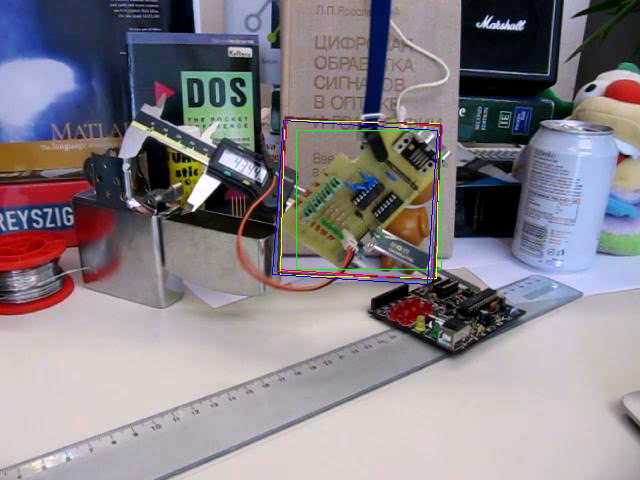
\includegraphics[width=0.19\linewidth]{imgs/dataset/d1.png}}
	\subfigure{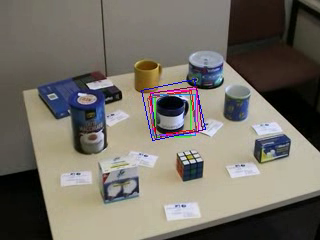
\includegraphics[width=0.19\linewidth]{imgs/dataset/d2.png}}
	\subfigure{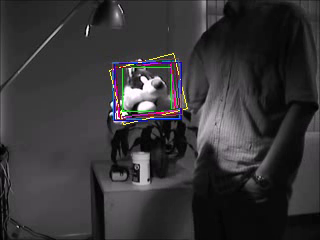
\includegraphics[width=0.19\linewidth]{imgs/dataset/d3.png}}
	\subfigure{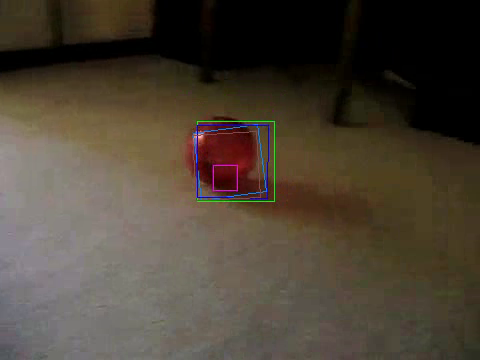
\includegraphics[width=0.19\linewidth]{imgs/dataset/d4.png}}
	\subfigure{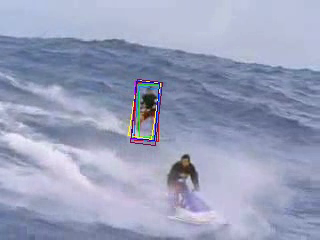
\includegraphics[width=0.19\linewidth]{imgs/dataset/d5.png}}}
	\vspace{-2mm}
\centerline{%
	\subfigure{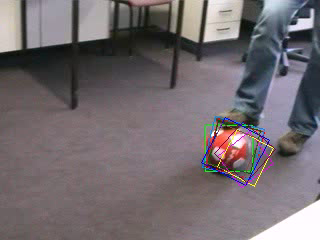
\includegraphics[width=0.19\linewidth]{imgs/dataset/d6.png}}
	\subfigure{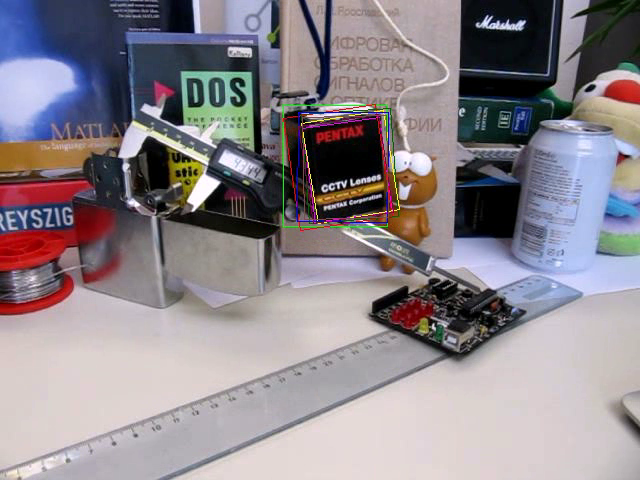
\includegraphics[width=0.19\linewidth]{imgs/dataset/d7.png}}
	\subfigure{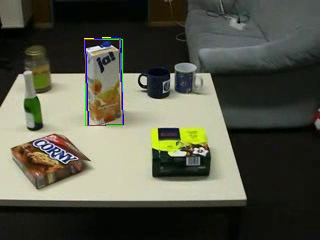
\includegraphics[width=0.19\linewidth]{imgs/dataset/d8.png}}
	\subfigure{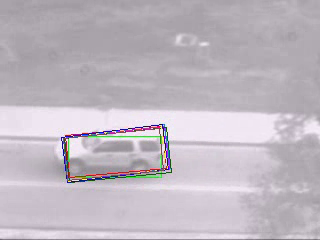
\includegraphics[width=0.19\linewidth]{imgs/dataset/d9.png}}
	\subfigure{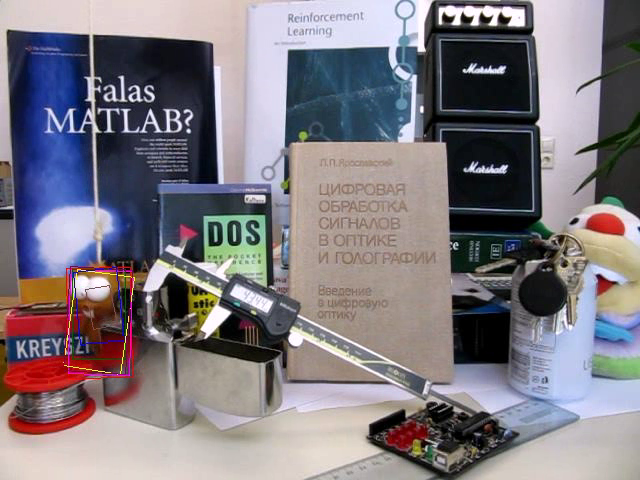
\includegraphics[width=0.19\linewidth]{imgs/dataset/d10.png}}}
\caption{The sequences of the dataset includes both indoor and outdoor scenarios with different light conditions.}
\vspace{-3mm}
\label{fig:data_example}
\end{figure*}


There are many publicly available datasets designed for tracking, however there is disagreement on how the data are stored. In order to facilitate the evaluation we collected the videos of different datasets and standardized how the data are stored. Fig.~\ref{fig:data_example} shows some examples. Each video is stored as a sequence of images while the ground truth, represented by an oriented bounding box, is saved in a comma separated value file where each row correspond to an image frame and contains 8 values representing the pairs x,y of each vertex of the box. The dataset will be available publicly, along with all the code to perform the experiments and compute the evaluation.

\subsection{Matching Evaluation Criteria}

\begin{figure}[b]
	%\vspace{-2mm}
	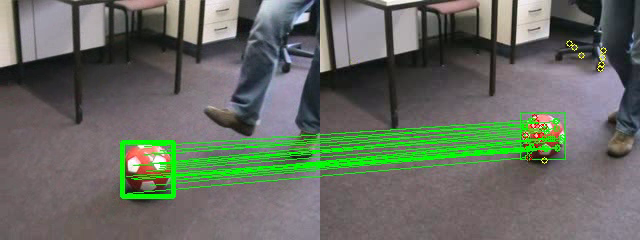
\includegraphics[width=0.95\linewidth]{imgs/matching.png}
\vspace{-2.5mm}	
\caption{Example showing how the matching precision is calculated. the image n the right shows the initial frame of the sequence. Matches in green are true positives. Circles in red are false positives. Yellow circles are false negatives, feature descriptors that are inside the object in the current frame but have a match with the background in our model.}
\label{fig:matching}
\end{figure}

Given as sequence of images $I_{1},...,I_{n}$ and the bounding box ground truth $gb_{1},...,gb_{n}$, we extract the set of target key-points descriptors $K_{1}$ from the first image of the sequence and we label all the key-points within $gb_{1}$ as descriptors of the object. For any subsequent image key-points $K_{t}$ are extracted and matched with $K_{1}$, generating a list of matches $M(i,j)_{k}$, where \textit{i} indicates a key-point descriptor of our target set $K_{1}$, and \textit{j} a descriptor of our test set. the test set is then labeled as follows:

\begin{equation}
K_{t}^{j} = 
\begin{cases}
\text{true positive}  \text{ if } K_{t}^{j} \in gb_{n} \land K_{1}^{i} \in gb_{1} \\
\text{false positive}  \text{ if } K_{t}^{j} \notin gb_{n} \land K_{1}^{i} \in gb_{1} \\
\text{false negative}  \text{ if } K_{t}^{j} \in gb_{n} \land K_{1}^{i} \notin gb_{1} \\
\end{cases}
\end{equation}

where the pair \textit{i,j} is determined by the matching result $M(i,j)_{k}$. Fig.~\ref{fig:matching} shows an example of how the key-points are labeled. The average ratio of true positives underlines the ability of a tracker to find the object and potentially recover from track loss. False negatives are feature descriptors that appear in the current frame but have no corresponding match in the initial test set $K_{1}$. This may happen due to drastic change in appearance of the object. The ratio of false positives is very important to consider since it indicates the average number of outliers that will be used to estimate the pose of the object, resulting in a bad pose estimation without employing additional filtering techniques. One widely used filtering technique consists in discarding all matched key-points if the ratio between the score of the best match and the second best match is below a certain threshold $\rho$. We define a key-point as ambiguous, if this criteria is not met. The  number of ambiguous true and false positives is then calculated to evaluate the distinctiveness of the descriptors and evaluate the influence of this common filtering technique on the results.

\subsection{Evaluating tracking precision}
\label{sec:accuracy}

\begin{algorithm}[h]
 \KwData{$I_{1},...,I_{n},b_{1}$}
 \KwResult{$b_{2},...,b_{n}$}
 $K_{1} \gets$ \textbf{extract\_points}($I_{1},b_1$)\;
 \For{$i \gets 2 : n$}{
   $K_{i}^{*} \gets$ track\_points($K_{i-1},I_{i-1},I_i$)\;
   $b_i \gets$ estimate\_pose($K_{i}^{*}$)\;
   $K_{i}' \gets$ \textbf{extract\_points}($I_{i},b_i$)\;
   $M \gets$ \textbf{match\_points}($K_{1},K_{i}'$)\;
   $K_{i} \gets$ merge\_keypoints($K_i^* ,  M$)\;
 }
 \caption{\label{alg:algorithm}Overview of the tracking algorithm used to compute the precision. The feature descriptors are employed in the steps in bold. }
\end{algorithm}

In order to measure the precision of the feature descriptors for tracking we employ a sparse key-point based tracker. The tracker requires a bounding box in the initial image of a sequence as initialization to extract feature descriptors that represent the \textit{model} of the object to track. The algorithm estimates the position of the object, represented as an oriented bounding box, with a combination of sparse optical flow and feature matching as shown in Alg.~\ref{alg:algorithm}. The original algorithm used ORB. We upgraded our algorithm making it more modular and able to cope with any possible feature descriptor. To estimate the precision we used the widely accepted overlap measure:

\begin{equation}
	\Theta (b_{t}, b_{gt}) = \frac{b_{t} \cap b_{gt}}{b_{t} \cup b_{gt}}
\end{equation}

where \textit{$b_{t}$} is the bounding box estimated by our tracker and
\textit{$b_{gt}$} is the bounding box provided by the ground truth. We define 
three precision requirements $\Upsilon$ (0.25, 0.5, 0.75) that indicates low, medium and high tracking accuracy. This is a more indicative evaluation compared to the overall accuracy. For instance, an overall value of 0.5 is ambiguous because it may indicate either a stable average accuracy around the value or a very precise evaluation in part of the video while poor in the rest.

The estimated object box \textit{$b_{t}$} is considered a true positive (TP) for a defined threshold of
accuracy $\Upsilon$ if:

\begin{equation}
\begin{cases}
b_{t} = TP  \text{ if } \Theta(b_{t}, b_{gt}) > \Upsilon \\
b_{t} = FP  \text{ otherwise }\\
\end{cases}
\end{equation}

The overall accuracy of the tracker for each precision requirement is calculated as:

\begin{equation}
\text{recall } = \frac{TP}{\text{TP } + \text{ FN}}
\end{equation}

%\missingfigure[figwidth=0.98\linewidth]{Figure showing the estimated bounding boxes and the ground truth to show the different behavior of trackers}

\subsection{Parameter setting}

All the descriptors require many parameters in order t be initialized properly. In order to evaluate the most fair comparison between them we decided to keep the values suggested by the original author of the descriptor or the implementation. However, there are some parameters that most of the feature descriptors shares that we set to the same value. The maximum number of features extracted is set to 2500 and the number of octaves is set to 4.



